\documentclass[a4paper]{article}
\title{\Huge{\textsc{Evolutionary Algorithms for Iterated Prisoner's Dilemma}}}
\usepackage[margin=3cm]{geometry}
\usepackage{graphicx}
\usepackage{wrapfig}
\usepackage{caption}
\usepackage[justification=centering]{caption}
\usepackage{amsmath}
\usepackage{subcaption}
\usepackage[export]{adjustbox}
\usepackage{enumerate}
\usepackage{url}
\usepackage{authblk}
\usepackage{float}
\usepackage{wrapfig}
\usepackage{setspace}
\usepackage{mdframed}
\usepackage{booktabs}
\usepackage{ragged2e}
\usepackage{subfig}

\graphicspath{{learnerPlots/}}

\def\changemargin#1#2{\list{}{\rightmargin#2\leftmargin#1}\item[]}
\let\endchangemargin=\endlist 

\DeclareMathSizes{10}{10}{10}{10}
\begin{document}

    \newgeometry{left=4cm,right=4cm,top=4cm,bottom=5cm}
	\begin{titlepage}
	    \begin{center}
	        \vspace*{5mm}
	        
	        \vspace{5mm}
	        {\Huge{\textsc{Evolutionary Algorithms}}}\\
	        \vspace{2mm}
	        {\huge{\textsc{for Infinite Prisoner's Dilemma}}}\\
	        \vspace{8mm}
	        {\large{Nishant Rai}}\\
			\vspace{3mm}
			
			{\normalsize{Department of Computer Science and engineering\\}}
	        \vspace{4mm}
        	\vspace{7mm}
	        \textbf{Abstract\\}
        	\vspace{4mm}
        	\noindent
{\justifying{The project deals with the problem of computing successful strategies for Iterated Prisoner's dilemma. We start off by discussing existing work in the area along with some results and popular methods used for computing efficient strategies. We simulate multiple results and also confirm previous findings and claims. We also show the relevance of choosing memory depth as three in Axelrod's experiments and provide arguments for the same. The discussed algorithms include Evolutionary Strategies and Reinforcement Learning (Which compute optimal and also adaptive strategies which perform well against multiple opponents). We propose new algorithms based on Reinforcement Learning to compute good strategies which perform well against a set of baseline algorithms (Including the extremely simple yet effective 'Tit for Tat'). This strategy is also compared against Axelrod's Evolutionary Strategy. We discuss Axelrod's Tournament and use a similar setup to decide the effectiveness of the computed strategies. The result section shows the superiority of the strategies computed using them. We also discuss the shortcomings and strengths of the algorithms.} \par}

			\vfill
			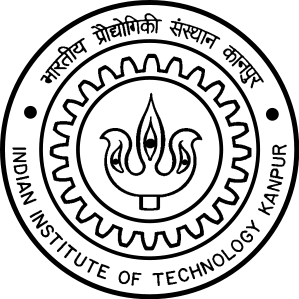
\includegraphics[width=0.25\textwidth]{iitklogo.png}\\[0.1in]
            \vspace{3mm}
	        {\Large{\textsc{ECO502A: Case Study}}\\}
			\vspace{3mm}            
            \normalsize{Under the guidance of Dr. Vimal Kumar\\}
            \vspace{1mm}
            {Indian Institute of Technology, Kanpur}
	    \end{center}
	\end{titlepage}
	\restoregeometry

	\tableofcontents
	
	\pagebreak	
	
	\section{Introduction}
	
	The Prisoner's Dilemma \cite{prisoner} is a classic problem in game theory, which is mainly a paradox demonstrating that two individuals acting in their own interest might choose an action which is worse off than any other. It has become a popular problem because there has been showing its similarity to real-world problems. The standard game is set up such that both players choose to protect themselves (Instead of cooperating) at the expense of their partner. Even though the thought process involved seems to be extremely logical, but both players eventually find themselves in a worse state than if they had cooperated with each other.\\
	
	We consider the following instance of Prisoner's Dilemma (Note that the essence remains the same). Players A and B have been arrested in connection with a crime. Both of them are put in a separate interview room and told that a deal may be available to them depending on whether each provides testimony against the other (Defects) or keeps silent (Cooperates). We assume that each  individual wants do as well as possible for only themselves (i.e. without any regard for the welfare of the other player). For further discussions, we denote the possible actions as $C_{x}$ and $D_{x}$ i.e. Player $x$ cooperating or defecting. The payoffs for the game are given in Table 1 below,

	\tabcolsep=0.51cm
	\begin{table}[H]
	\centering
	\begin{tabular}{|c|c|c|}
	\hline
					& $C_{B}$           		& $D_{B}$ 					\\ \hline
	$C_{A}$  		& (3,3) 		 			& (0,5)         			\\ \hline
	$D_{A}$			& (5,0)           			& (1,1)            			\\ \hline
	\end{tabular}
	\caption{Payoff matrix for the Prisoner's Dilemma}
	\end{table}
		
	For ease of discussion afterwards, we define the following terms \cite{optimalipd} based on the actions chosen by the players (They are described in Table 2),
	\begin{itemize}
		\item T : \textbf{Temptation} for unilateral defection
		\item R: \textbf{Reward} for mutual cooperation
		\item P : \textbf{Punishment} for mutual defection
		\item S: \textbf{Sacrifice} for unilateral cooperation	
	\end{itemize}
	
	\begin{table}[H]
	\centering
	\begin{tabular}{|c|c|c|}
	\hline
					& $C_{B}$           		& $D_{B}$ 					\\ \hline
	$C_{A}$  		& (R,R) 		 			& (S,T)         			\\ \hline
	$D_{A}$ 		& (T,S)           			& (P,P)            			\\ \hline
	\end{tabular}
	\caption{State definitions for the Prisoner's Dilemma}
	\end{table}

	As discussed earlier, we can conclude that the moves chosen by the players would be $(D_{A},D_{B})$. This can be termed as the Nash Equilibrium of the game. An interesting variant of the classical prisoner's game arises when the game is repeated multiple times. It is termed as Iterated Prisoner's Dilemma. The situation becomes even more interesting when the game satisfies the following conditions,
	\begin{enumerate}
	\item The winner is the player with the highest score in the end.
	\item The number of moves should 'not' be known to the two players.
	\item Usually, there are many players in the fray, and there is a Round Robin Tournament among all the players - the player with the highest score wins.		
	\end{enumerate}
	
	Due to the fact that the players do not know the number of repetitions of the game, thus it becomes equivalent to playing the game infinite times.	This is the game we will be studying in this Case study: The Infinitely Repeated Prisoner's Dilemma (Or Infinite Prisoner's Dilemma (IPD)).
	
	\section{Existing Work}
	
	There has been a huge amount of work in the area of Prisoner's Dilemma (And its variants) \cite{existA}, \cite{existB}, \cite{existC}; on both theoretical and practical implications and applications. In the case of Infinite Prisoner's Dilemma, it can be argued that Axelrod \cite{axelrod} has been the most influential researcher in the area. His original work set the stage for a regularized study in terms of tournaments amongst multiple strategies. The surprising results of Axelrod's work \cite{axelrod} has fueled a lot of discussions and further works \cite{existA}, \cite{optimalipd}. In his original work, two tournaments based on IPD were undertaken; which later defined the methods by which IPD strategies ought to be compared. In the process, he invited professional game theorists to submit programs for playing a computer-based Infinite Prisoner's Dilemma. His work has also been extremely influential in other studies (Especially in demonstrating the effectiveness of Evolutionary Algorithms in unconventional applications).
	
	Later, Axelrod used a Genetic Algorithm (GA) \cite{genetic}, an artificial intelligence technique (Inspired by biological evolution), to simulate agent learning. The algorithm uses operators such as mutation and crossover (Derived from evolution). Crossover is a genetic operator used to vary the chromosomes from one generation to the next (i.e. Induce diversity and evolution). It is simply a process of taking more than one parent solutions and producing a child solution from them. Mutation is an operator used to maintain genetic diversity from one generation to the next. In investigating evolutionary strategies, Axelrod considered a set of strategies that is deterministic (fixed) and uses results (histories) of the past 'three' moves (Discussed later) to determine the best move for the next turn.
	
	There has been work which adapt and extend the same approach showing the effectiveness of their approach \cite{existC}, \cite{optimalipd}. One of the shortcomings of evolved strategies is the fact that the optimization algorithms used to compute good strategies are not able to effectively search the complete solution space. This leads to surprisingly poor strategies as we increase the history considered. We study the effect of this in later sections.
	
	Note that most of the strategies in these works are history dependent. In other words, such an a class will consist only of memory-based strategies. However, previous works \cite{pavlov} also show the existence of alternative representation of (effective) strategies. Kraines et al \cite{pavlov} showed that 'Pavlovian' strategies are able to support the evolution of cooperation in tournaments where players are making errors. Pavlovian strategies are similar to Tit for Tat in the sense that they are extremely simple. If your opponent cooperated with you on the last round, repeat your last move; otherwise, switch your move. Its biggest advantage is that, unlike TFT, it is relatively prone to errors and can bounce back from a $D-D$ stalemate. This has been explored in detail by Kraines et al.
	
	\section{Axelrod's Tournament}

	We discuss details of Axelrod's Tournament \cite{axelrod} in detail in this section. Axelrod held a tournament of various strategies for the prisoner's dilemma. A number of game theorists submitted strategies which were simulated using computers. The tournament was a round robin tournament i.e. programs played games against each other repeatedly.\\
	The results were extremely interesting and led to many discussions eventually. Some of the strategies submitted were:
	\begin{itemize}
	\item \textbf{Always Defect}: This strategy defects on every turn. This is what game theory advocates. It is the safest strategy since it cannot be taken advantage of. However, it misses the chance to gain larger payoffs by cooperating with an opponent who is ready to cooperate.
	\item \textbf{Always Cooperate:} This strategy does very well when matched against itself. However, if the opponent chooses to defect, then this strategy will do badly.
	\item \textbf{Random:} The strategy selects its move randomly i.e. cooperates and defects 50\% of the time.
	\item \textbf{Tit for Tat:} Cooperates on the first move, then simply copies the opponent's last move.
	\end{itemize}
	
	All of these strategies act without any knowledge of the future behavior of the opponent. Therefore, they cannot take advantage of knowing the opponent's previous moves and figuring out its strategy (There was actually a bugged tournament conducted later on, which suffered from this flaw and was exploited effectively by the winner). The winner of Axelrod's tournament was the extremely simple 'Tit for Tat' strategy. As mentioned earlier, the strategy cooperates on the first move, and then does whatever its opponent has done on the previous move. Thus, when matched against the all-defect strategy, 'Tit for Tat' strategy always defects after the first move. When matched against the all-cooperate strategy, 'Tit for Tat' always cooperates. This strategy has the benefit of both cooperating with a friendly opponent, getting the full benefits of cooperation, and of defecting when matched against an opponent who defects. When matched against itself, the 'Tit for Tat' strategy always cooperates.\\
	'Tit for Tat' relies on the assumption that its opponent is trying to maximize his score. When paired with a mindless strategy like 'Random', 'Tit for Tat' sinks to its opponent's level. For that reason, 'Tit for Tat' cannot be called the 'best' strategy. It must be realized that there really is no 'best' strategy for prisoner's dilemma. Each individual strategy will work best when matched against a 'worse' strategy. In order to win, a player must figure out his opponent's strategy and then pick a strategy that is best suited for the situation.
	
	\subsection{Features of Successful Strategies}

A strategy (pure) for a player in a particular game is a plan describing what move that player should take in each possible situation (information state) that might arise for him.
In Axelrod’s IPD tournaments, strategies exhibiting the following four properties (As observed by Axelrod in \cite{axelrod}) tended to be more successful (i.e., to accumulate higher total payoffs), with the clear-cut winner being the Tit-for-Tat strategy.
	\begin{itemize}
		\item \textbf{Niceness}: Never be the first to defect.
		\item \textbf{Provocability}: Get mad quickly at defectors and retaliate.
		\item \textbf{Forgiveness}: Do not hold a grudge once you have vented your anger.
		\item \textbf{Clarity}: Act in ways that are straightforward for others to understand.
	\end{itemize}

	We study whether these traits are actually useful or not in the result section. We try to see  if the computed strategies have the mentioned features.
	
	\subsection{Axelrod Strategies}	

As we have seen earlier that 'Tit for Tat' turned out to be the winner in Axelrod's tournament even though it can perform worse against many opponents (e.g. Random). Axelrod set out to find other simple strategies with similar or greater power. This section describes the procedure followed by Axelrod to compute a new strategy.
Axelrod adopted a simple but elegant way for encoding strategies, and then used a single-objective evolutionary algorithm to obtain optimal strategies. His encoding scheme has remained a standard way of handling the IPD problem and is described below. We also adopt a similar encoding scheme to compute optimal strategies for the game. Axelrod's method had the following features,
	\begin{itemize}
	\item The next move depends upon the behavior of both the parties during previous three (In general k, termed as memory length in this paper) moves.
	\item We have four possibilities for the previous move, which are as follows,
	\begin{itemize}
		\item CC or R for Reward
		\item CD or S for Sacrifice
		\item DC or T for Temptation
		\item DD or P for Punishment
	\end{itemize}		
	\item We code the particular behavioral sequence as a 3-letter string.	
	\item We then use the 3-letter sequence to generated a number between 0 and 63 (i.e. $4^{3} = 4^{k}$) by interpreting it as an integer base 4 (Since there were 4 possibilities for each turn).
	\item Strategy string : 64-bit binary string of C's and D's where he $i^{th}$ bit corresponds to the $i^{th}$ behavioral sequence.
	\end{itemize}

	The following \textbf{critical} points should be observed,
	\begin{itemize}
	\item The behavior of the player is undefined in the first three moves of the game (Since we do not have histories of the game).
	\item We also add six bits to the encoding to specify a strategy's premises, i.e. assumption about the pre-game behavior (or alternatively behavior in the first three iterations).
	\item Together, each of the 70-bit strings represent a particular strategy (i.e. State-action codes)	
	\end{itemize}		
	
	Note that we can vary the history considered by the strategy, which consequently changes the memory required for the strategy encoding. This also raises the computational cost as mentioned earlier. We study the effect of memory in the result section.
	
	\section{Motivation}
	
	As discussed in the previous section, Axelrod's encoding can be used to define a strategy. We decide to use Evolutionary Algorithms to compute the optimal (Axelrod) strategy because the total number of all possible strategies very high (i.e. $2^{70}$). If we perform an exhaustive search, it will take a huge amount of time (A couple billion years or more!). We do not seek help from standard optimization procedure since the fitness function required is not continuous or differentiable, thus classical methods will not work. Hence, genetic (evolutionary) algorithms are a good choice.

	\section{Axelrod Strategies using Evolutionary Algorithms}

	As mentioned earlier, Axelrod's approach involved maximizing the self score using a Single Objective Genetic Algorithm. We try to recreate the results and study the effectiveness of the approach proposed by Axelrod. There has also been work \cite{optimalipd} which proposes optimizing multiple objectives simultaneously (i.e. Self Score and Opponent score) NSGA-II \cite{nsga}, \cite{debmulti} algorithm. It has been claimed that the latter works better, thus we compare the performance of both the algorithms to validate the claims and get more details related to their effectiveness.
	
	The intuition for using another objective (i.e. Opponent score) is that maximizing our own score is not the only way to win the game. The game can also be won if we minimize the score of the opponent. Thus, minimizing the opponent score might indirectly help us win the game.
	
	A flaw of such evolved strategies is there non-adaptive nature. Note that the strategies learned using the mentioned algorithms would be fixed i.e. they can not change their behavior based on the opponent's behavior. Also, the computed strategies work well only with the strategies they are trained with (or exposed during the evolution). Their behavior with fresh strategies is disappointing to say the least. To counter this drawback, we study and propose a few adaptive strategies which adapt to the opponent, and learn the best behavior given sufficient time.
	
	\section{Proposed Algorithms}
	
	The previous section motivates us to search for strategies which are able to adapt to new opponents. This section discusses a topic named Reinforcement learning, which focuses on algorithms which make a player (computer) learn how to play a new game (A game to which it has never been exposed before).
	
	\subsection{Reinforcement Learning for Adaptive Strategies}
	
	\subsubsection{Introduction}
	
	Let's consider a basic game to appreciate the power of reinforcement learning. Let us play the following game (Termed as n-armed bandit). We have $n$ slot machines, each of which gives some unknown (yet constantly distributed, more later) payoff once it is played. Assume that there is no cost associated with playing the game. Thus, we have n possible actions and at each play ($k$), we can choose a single slot machine to play at. After taking an action $a$, we receive a reward $R_{k}$ (reward at turn $k$). Each slot machine has a unique probability distribution of payouts (rewards).\\
	
	For example, if we have 10 slot machines, let slot \#3 give an average payoff of 9 while slot \#1 gives an average payoff of 4. Note that since the reward at each play is distributed according to some probability distribution, it is possible that slot \#1 might give us a reward of 1 on some turn. But on average, slot \#1 would give us reward close to 4. Thus, a reasonable strategy would be playing random moves a few times i.e. choosing different slots and observing our rewards for each action. Then we might prefer choosing the slot with the largest observed average payoff. Thus we will need a value which gives us an idea of the expected payoff by choosing move $a$ (Based on our previous turns), let's call this expected reward $Q_{k}(a)$. $Q_{k}(a)$ is a function which accepts action $a$ and gives the expected payoff for the action. Formally we can write it as,
\begin{equation}
Q_{k}(a) = \frac{R_{1} + R_{2} + \cdots + R_{k}}{k}
\end{equation} 

Simply put, the expectation for reward at turn $k$ for move $a$ is the mean of all the previous rewards we've received for taking action $a$. Thus, our previous moves and rewards influence our future actions.
This discussion also introduces the concept of exploration and exploitation. Note that our strategy needs to include some amount of exploitation (i.e. simply choosing the best slot based on what we know so far) and some amount of exploration (i.e. Occasionally choosing random moves to learn more about the nature of the game). This balance between exploration and exploitation leads to the Explore-Exploit dilemma \cite{expexp}.

Thus a simple adaptive strategy	can be simply choosing the (seemingly) best move (i.e. the one with the highest payoff) with probability $p$ and choosing a random move with $1-p$ (This accounts for exploration. We discuss multiple variants for reaching a balance between exploration and exploitation and compare the results in the later sections.

	\subsubsection{Adaptive Strategy: Variant A}

	The first variant of the adaptive strategy is an extremely simple algorithm which just chooses the (seemingly) best move (i.e. the one with the highest payoff) with probability $p$ and choosing a random move with $1-p$ (This accounts for exploration). It is the same version we've mentioned above. There are a few flaws in this variant namely, non varying exploration which is actually desired (Since, we would want more exploration initially and then decrease our exploration once we are sure). Thus, the results for this variant are very poor and have not been shown due to space constraints.
	
	\subsubsection{Adaptive Strategy: Variant B}
	
	The second variant builds upon the 	flaws of variant A and includes varying thresholds for $p$. $p$ decreases as we keep exploring, thus when we become sure about the best response, we shouldn't explore much. The related results for this variant are shown in the result section.
	
	\subsubsection{Adaptive Strategy: Variant C}
	
	This variant further modifies the exploration part, we mainly use a softmax probability during the exploratuon part. The effect and motivation are given below. (The examples are inspired from \cite{reinf}).\\
	
	\textbf{Softmax Action Selection:} Let's consider another problem, a new doctor specializes in treating patients with a particular disease. She has $n$ treatment options of which she can choose one to treat each patient she treats. For some reason, all she knows is that these $n$ treatments have different efficacies and risk-profiles for treating heart attacks, and she doesn't know which one is the best yet. We could still use the same $p$ greedy algorithm mentioned above, however policy of randomly choosing a treatment once in a while might prove fatal. Here, randomly treatments could result in patient death. Thus, we would want not to choose the worst treatment but still have some ability to explore our options to find the best one.\\
	
	This is exactly where softmax selection fits in. Instead of choosing an action randomly (during exploration), softmax helps us get a probability distribution on our moves. The option with the largest probability would be equivalent to our best move from the above variants, but we also have some idea about the $2^{nd}$ and $3^{rd}$ best moves. Thus, we can randomly choose to explore other options while avoiding the very worst options. Formally, the softmax equation,
\begin{equation}
	P(a) = \frac{e^{Q_{k}(a)/c}}{\sum_{i=0}^{n} {e^{Q_{k}(i)/c}}}
\end{equation} 
	
	The parameter $c$ scales the probability distribution of the moves. A high $c$ will push the probabilities to be very similar, while a low $c$ will magnify the differences in probabilities. This parameter plays a critical role in the final performance of the strategy as will be seen in future sections.
	
	\pagebreak	
	
	\section{Experiments}
	
	Both Single Objective Evolutionary Algorithm and Multi Objective Evolutionary Algorithm (MEA) are used for getting optimal strategies. The discussed strategies are evaluated in the later sections as discussed below.\\
	We describe the rough structure of the evolutionary algorithms. In each generation, a certain number (referred to as population size) of strategies are generated, and each strategy was made to play against \textbf{n} other players. Each game consisted of \textbf{p} moves. Then the next generation is created using a recombination operator involving the best strategies from the earlier one. The payoff matrix is the same as shown in Table 1. The details of the \textbf{n} other players have been given in the section: \textit{Baseline Strategies}.

	\subsection{Baseline Strategies}
	
	The baseline strategies used in the experiments are as follows \cite{optimalipd},
	\begin{enumerate}
	
	\item \textbf{Always Cooperate:} Cooperates on every move
	\item \textbf{Always Defect:} Defects on every move
	\item \textbf{Tit for Tat:} Cooperates on the first move, then simply copies the opponent's last move.
	\item \textbf{Suspicious Tit for Tat:} Same as Tit for Tat, except that it defects on the first move
	\item \textbf{Random:} Makes a random move.
	\item \textbf{Cyclic CCD:} Plays C, C, D periodically.
	\item \textbf{Tit for Two Tats:} Cooperates on the first move, and defects only when the opponent defects two times.
	\item \textbf{Soft Majority:} Begins by cooperating, and cooperates as long as the number of times the opponent has
cooperated is greater than or equal to the number of times it has defected, else it defects.
	\item \textbf{Hard Majority:} Defects on the first move, and defects if the number of defections of the opponent is greater than or equal to the number of times it has cooperated, else cooperates.
	\item \textbf{Hard Tit for Tat:} Cooperates on the first move, and defects if the opponent has defects on any of the previous three moves, else cooperates.
	\item \textbf{Prober:} Plays D, C, C initially. Defects forever if opponent cooperated in moves 2 and 3. Otherwise plays Tit for Tat.	
	\end{enumerate}
	
	\subsection{Tournament Setup}
	
	The tournament setup is inspired by Axelrod's initial study. It consists of a round robin tournament amongst all the strategies where each game is played for 200 turns. The whole tournament is repeated a few times (10 times in our experiments) to lessen the effect of randomness.

	\section{Results for Evolutionary Algorithm}

	\subsection{Evolution Statistics}

	\subsubsection{Single Objective Genetic Algorithm}	

	\begin{wrapfigure}{R}{0.45\textwidth}
	\centering
	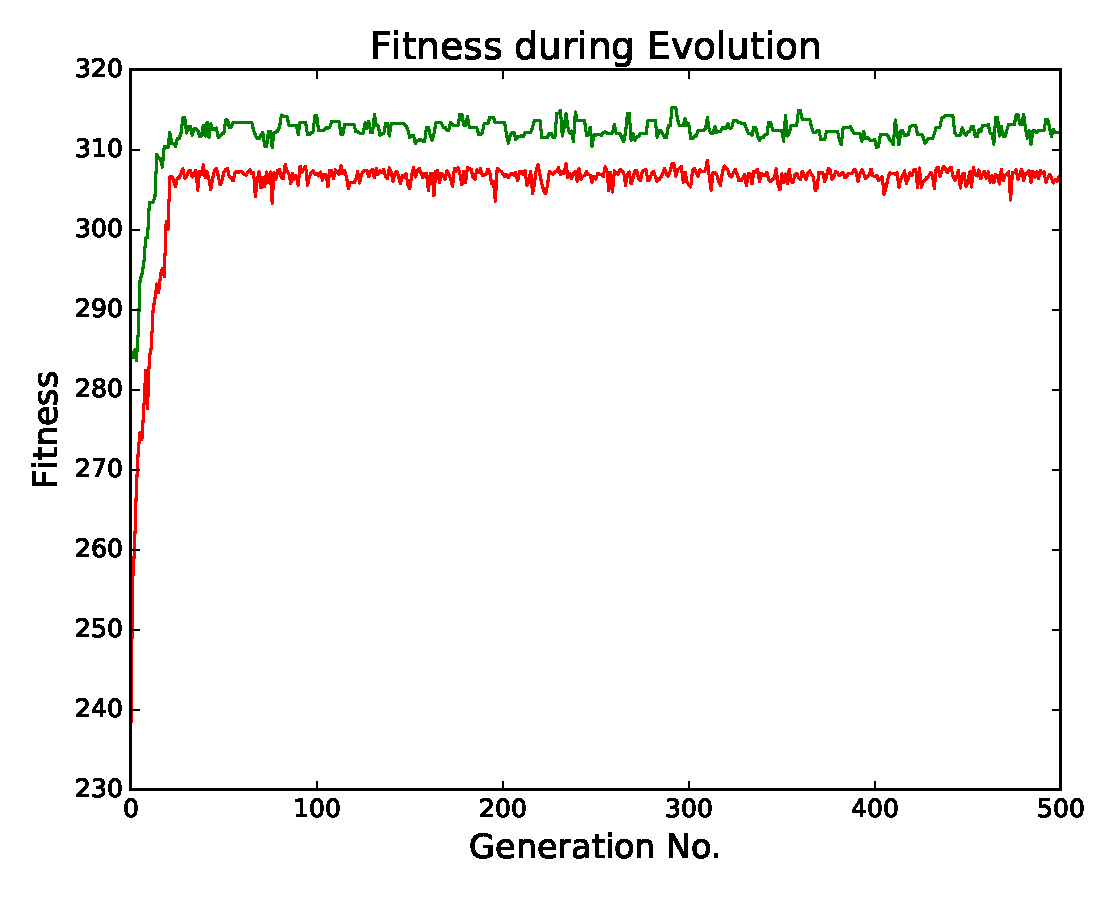
\includegraphics[width=0.43\textwidth]{singFitPlot.eps}
	\caption{\footnotesize{Fitness of Population during Evolution}}
	\end{wrapfigure}
	The single-objective Evolutionary Algorithm used is the same as used by Axelrod in his initial study. As done earlier, the fitness i.e. self-score of the player is maximized during evolution. For the experiment, the population size was fixed at 60. The results obtained when the evolutionary algorithm is run for 500 generations is shown in figure.\\
	We show the maximum and average fitness of the population. As we can see the population achieves the final value extremely quickly (Under 50 iterations). The fluctuations caused in between are a result of the mutations introduced in the population (Something inherent in Evolutionary Algorithms).\\
	After 500 generations the maximum fitness amongst all the samples in the population is around 312, which is even higher than the benchmark score (300) \cite{dawkins}. This shows the superiority of the Evolutionary strategy and is also in line with the results obtained by Axelrod. When this strategy is pitted against other strategy in an Axelrod-like tournament, the evolved strategy emerges as a clear winner (By a huge margin). The results are discussed in later sections.	

	\subsubsection{Multi Objective Genetic Algorithm}
		
	\begin{wrapfigure}{R}{0.45\textwidth}
	\centering
	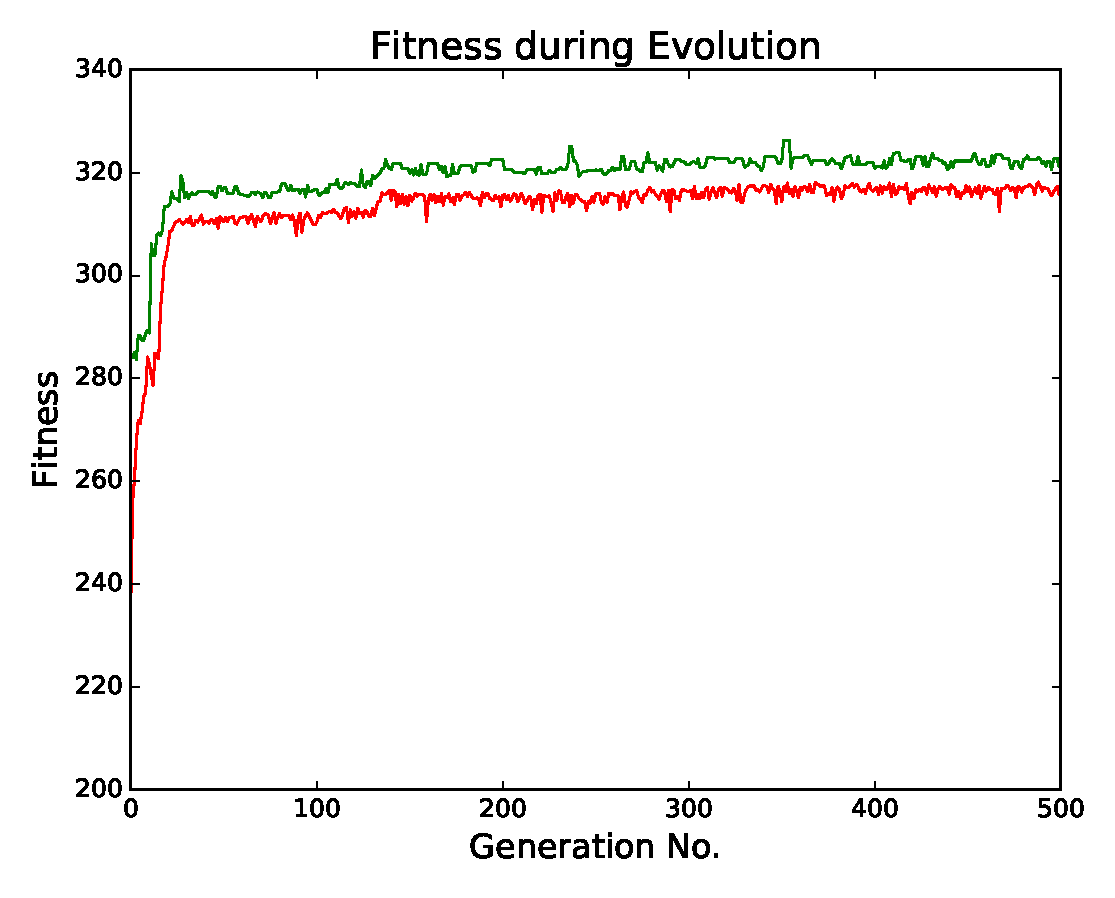
\includegraphics[width=0.43\textwidth]{multFitPlot.eps}
	\caption{\footnotesize{Fitness of Population during Evolution}}
	\end{wrapfigure}
	
	Instead of just maximizing our own score as proposed by Axelrod \cite{axelrod}, we perform another experiment in which along with maximizing our self score we also try to reduce the opponents score. The intuition for this can be seen from the payoff matrix of the game and has been discussed earlier.\\
	We used a Multi-Objective Evolutionary Algorithm (NSGA-II) \cite{nsga} to compute the strategy. For the experiment, the population size was fixed at 60. The results obtained when the evolutionary algorithm is run for 500 generations is shown in figure. We show the maximum and average fitness of the population. The behavior of evolution mostly remains similar to the previous case. But we can see that the final value obtained \textit{(321)} in this case is higher than the Single Objective counterpart \textit{(312)}, which further motivates the benefit of using a multi-objective optimization algorithm.\\

	To further demonstrate the evolution, we plot the initial and final strategies obtained in Figure 3. The blue crosses represent the initial randomly initialized strategies. The red pluses represent the final evolved strategies, it can be easily seen that the initially random population slowly approaches the 'optimal' region. The out of place red members in the final evolved population are the mutated individuals.
	
	\subsection{Effect of Memory on Strategies}
	
	Axelrod performed his experiments assuming a memory length of \textbf{3}. We perform our experiments with multiple memory lengths to gain insight whether it is in fact optimal. The results are shown in the following table,
	
	\begin{table}[H]
	  \begin{center}
	    \begin{tabular}{c|c|c}
	      \toprule
	      \textsc{Memory Length} & \textsc{Self Score} & \textsc{Encoding Size}\\
	      \midrule
	      1 & 280.18 & 6\\
		  2 & 291.36 & 20\\
		  \textbf{3} & \textbf{314.27} & \textbf{70}\\
		  4 & 281.72 & 264\\
		  5 & 284.09 & 1034\\
		  6 & 296.18 & 4108\\		  
		  \bottomrule
	    \end{tabular}
	    \caption{\textsc{Effect of Memory}}
	  \end{center}
	\end{table}  

	\begin{figure}[H]
	\centering
	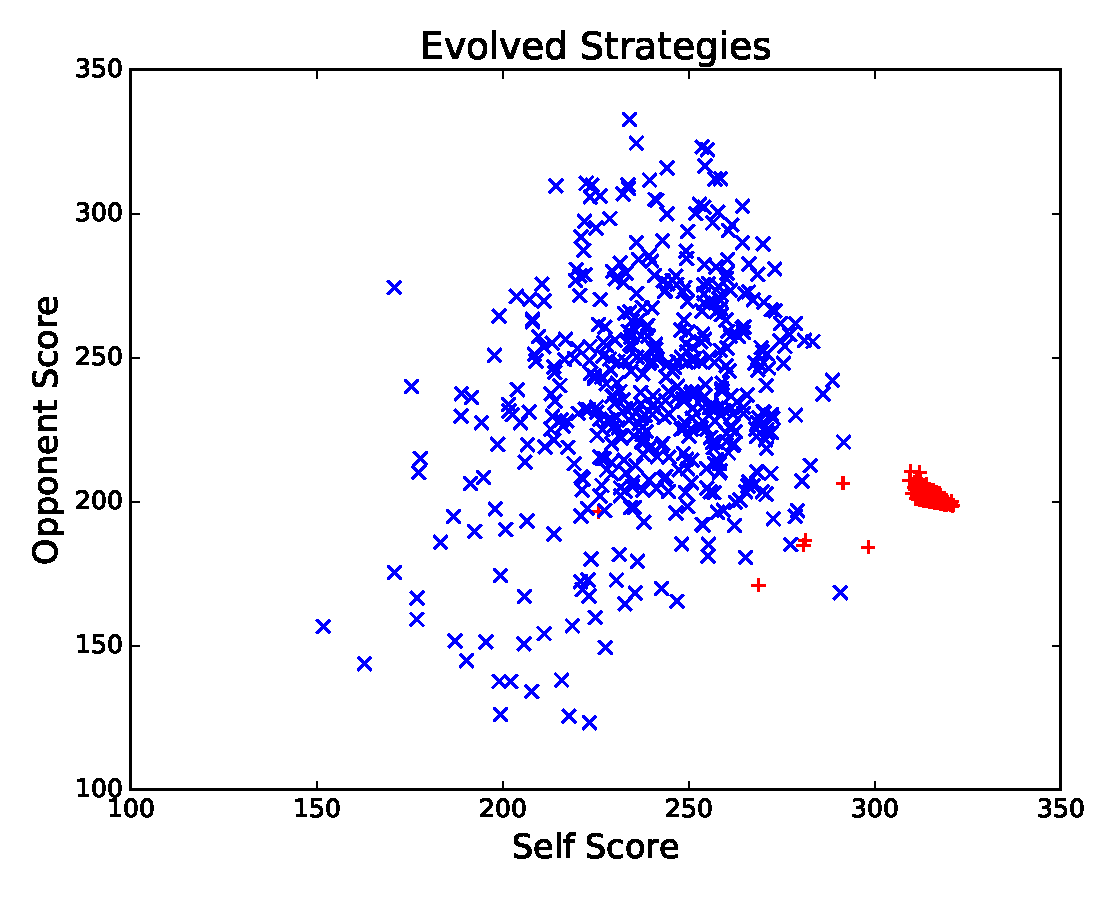
\includegraphics[width=0.65\textwidth]{evolvePlot.eps}
	\caption{{Distribution of Final Evolved Strategies and the Initial Randomly initialized Strategies}}
	\end{figure}

	As we can see in the table shown above (Table 3). As we increase the memory length, an interesting trend is observed. At first, the memory increases till an optimum value (i.e. 3) then it suddenly decreases. Then, after the sudden decrease it gradually increases once again.\\
	
	Notice that ideally, higher memory must result in better performance. Because it's trivial to show that the set of strategies using memory $n$ must be a subset of the set of strategies using memory $n+1$. But unfortunately this is the opposite of what is observed in the experiments. We suspect that the reason for poor performance despite the earlier mentioned fact is the limitations of the Genetic Algorithm. As memory length increases, the corresponding solution space also increases exponentially. This results in the algorithm being prone to get stuck in local minimas. It also means that the Genetic Algorithm would require more generations (iterations) to arrive at a reasonable solution. Thus, the value proposed by Axelrod (i.e. 3) seems to be the optimal memory length considering the trade-off between Computational Power and Performance.\\
	
	This trade-off can be loosely formalized using two indicator functions $f_{p}(k)$ (Represents the ideal performance at memory $k$) and $f_{c}(k)$ (Represents the computational cost for computing strategies of memory $k$). On the basis of the earlier discussions, both $f_{p}(k)$, $f_{c}(k)$ would be increasing with k.
	
	\noindent
	The effective efficiency of the learned strategy can be approximated as $(f_{p}(k) - f_{c}(k))$
	 
	 The exact formula of $f's$ is difficult to determine but a rough estimate regarding the behavior of the functions can be inferred from the table shown above. 

	\subsection{Tournament amongst strategies}

	We conduct an Axelrod-like tournament amongst the mentioned strategies to compare and evaluate them. The baseline strategies used are mentioned in the earlier sections. The numbers (scores) shown represent the average score received in each move (This is a popular metric used in literature \cite{optimalipd} along with the baseline score \cite{dawkins}). Remember that 3 is the payoff when both players always cooperate.

	\subsubsection{Multi Objective Strategy Vs Others}

	In this setup we conduct a tournament between the strategy computed using the Multi Objective GA and the baseline strategies. The best performer has been highlighted in bold text. The average score refers to the average payoff per turn.

	\begin{table}[H]
	  \begin{center}
	    \begin{tabular}{c|c}
	      \toprule
	      \textsc{Player} & \textsc{Average Score}\\
	      \midrule
			Cooperator & 2.091\\
			Defector & 1.799\\
			Cycler CCD & 2.339\\
			Hard Go By Majority & 2.023\\
			\textbf{Multi Objective Strategy} & \textbf{3.183}\\
			Soft Go By Majority & 2.418\\
			Hard Tit For Tat & 2.317\\
			Tit For 2 Tats & 2.304\\
			Suspicious Tit For Tat & 2.269\\
			Random: 0.5 & 2.244\\
			Tit For Tat & 2.627\\
			Prober & 2.510\\
		  \bottomrule
	    \end{tabular}
	    \caption{\textsc{Tournament Results}}
	  \end{center}
	\end{table}  

	Notice the high performance of 'Tit for Tat' strategy which confirms Axelrod's result.

	\subsubsection{Single Objective Strategy Vs Others}

In this setup we conduct a tournament between the strategy computed using the Single Objective GA and the baseline strategies. The best performer has been highlighted in bold text. The average score refers to the average payoff per turn.
	
	\begin{table}[H]
	  \begin{center}
	    \begin{tabular}{c|c}
	      \toprule
	      \textsc{Player} & \textsc{Average Score}\\
	      \midrule
			Cooperator & 2.089\\
			Defector & 1.807\\
			Cycler CCD & 2.333\\
			Hard Go By Majority & 2.037\\
			\textbf{Single Objective Strategy} & \textbf{3.159}\\
			Soft Go By Majority & 2.426\\
			Hard Tit For Tat & 2.319\\
			Tit For 2 Tats & 2.304\\
			Suspicious Tit For Tat & 2.273\\
			Random: 0.5 & 2.273\\
			Tit For Tat & 2.630\\
			Prober & 2.500\\
		  \bottomrule
	    \end{tabular}
	    \caption{\textsc{Tournament Results}}
	  \end{center}
	\end{table}
	
	The same trend as earlier follows in this case too. But also observe that the average score obtained by the Multi-Objective Strategy is higher than that of the Single Objective strategy. Which supports the inclusion of multiple objectives during optimization.d

	\subsubsection{Tournament with all strategies}
	
In this setup we conduct a tournament consisting of both the evolutionary strategy and the baseline strategies. The best performer has been highlighted in bold text. As earlier, the average score refers to the average payoff per turn.	
	
	\begin{table}[H]
	  \begin{center}
	    \begin{tabular}{c|c}
	      \toprule
	      \textsc{Player} & \textsc{Average Score}\\
	      \midrule
			Cooperator & 2.043\\
			Defector & 1.737\\
			Cycler CCD & 2.179\\
			Hard Go By Majority & 1.977\\
			\textbf{Multi Objective Strategy} & \textbf{3.051}\\
			Soft Go By Majority & 2.356\\
			Hard Tit For Tat & 2.375\\
			Tit For 2 Tats & 2.235\\
			{Single Objective Strategy} & {3.045}\\
			Suspicious Tit For Tat & 2.331\\
			Random: 0.5 & 2.201\\
			Tit For Tat & 2.661\\
			Prober & 2.551\\
		  \bottomrule
	    \end{tabular}
	    \caption{\textsc{Tournament Results}}
	  \end{center}
	\end{table}  

	It can be seen that the Multi Objective Strategy performs slightly better than the Single counterpart. This reaffirms the superiority of the Multi Objective strategy over the Single Objective one.
		
	\subsection{Behavior of the Evolved strategies}

	We choose a few individuals out of the evolved population randomly and compare the strategies obtained. We mention some of the interesting traits found common in all the strategies. We also try to relate the trends observed in these strategies to the desirable qualities (Proposed by Axelrod \cite{axelrod}) required for successful strategies (Mentioned in previous sections). Some of the trends noted in the strategies are as follows,
	\begin{itemize}
	\item \textbf{PPP (0) :} In this situation both the players have been defecting over the previous three moves. Since both players were defecting previously, defecting again would be a good choice to minimize the damage and prevent the opponent's score to increase.
	\item \textbf{PPT (1) :} In this case, the opponent defected on the first two moves, but cooperated in the third move, while player 1 defected in all the three moves. Thus, we should continue to exploit the 'foolishness' of the opponent and defect in the next move too (Expecting the opponent to cooperate).
	\item \textbf{PTP, PTT (4, 5) :} Here, all of the given cases are similar to the previous case, which means defecting would be the best choice (To exploit the 'foolish' opponent).
	\item \textbf{PRR (15) :} Here, the opponent has cooperated for the last few moves, so in order to gain more points defecting will be a good choice. But, note that this may make the opponent distrustful.
	\item \textbf{TPT, TTT (17, 21) :} All the given cases are similar to the previous case, which means defecting would be the best choice (To exploit the 'foolish' opponent).
	\item \textbf{TTP (20) :} Here, the opponent was cooperating with us initially. But it didn't in the last move, which shows that trust has been lost and the best move would be to defect again.
	\item \textbf{TRR (31) :} After being betrayed, we and the opponent both start cooperating. Thus, to exploit this relationship it would be best to defect next.
	\item \textbf{STT (37) :} This case is quite similar to the 'foolish' opponent cases discussed above. So, the best choice is to defect.
	\item \textbf{SRR (47) :} After being betrayed, we and the opponent both start cooperating. Thus, we should continue cooperating. Note the difference between 31 and 47. Even though the last two turns (histories) are the same, the next action is completely different. It can be speculated that this is due to the fact that in 31, the opponent trusts us easily (Since it cooperated after being betrayed). So, we can betray it again, hoping that it won't mind. But in this case, we are not aware of the opponent's behavior (Since we were betrayed here).
	\item \textbf{RTR (55) :} This case is again similar to the 'foolish' opponent case. In this case, the opponent trusts us easily. So, exploiting this behavior would be the best.
	\item \textbf{RRT (61) :} Here, both players have cooperated in the initial two moves and we've exploited it in the last turn. So, now that trust has been lost it would be better to defect.
	\item \textbf{RRR (63) :} In this case, both players have cooperated in the last few moves. So, the best move would be to continue cooperating (So that we don't lose trust).
	\end{itemize}
	
	We observe that the strategies learned are 'Nice', 'Provocative' and 'Clear'. Because, in case both the players are cooperating, we do not defect and break trust i.e. not the first one to defect (Niceness). We also lash back at a defecting opponent accordingly and not be misused by him (Provocative).  We 'might' also say that our moves are pretty 'Clear' and give a straight signal to the opponent (We say it is clear on the basis of the discussion above i.e. the idea behind most moves was explained using simple-straightforward logic).\\
	
	A deviation from Axelrod's features occurs in case of 'Forgiveness'. We do not easily forgive the opponent, which is in a way a nice feature (But fails in case of a few strategies i.e. Tit for Tat). We propose another feature named 'Exploiter', which basically means being able to exploit a foolish opponent. It's easy to see that exploiting the opponent is the major source of points (payoffs) in the game.
	
	\section{Results for Adaptive Strategies}

	In this section we discuss various results related to the adaptive strategies and study the effect of parameters and also the performance of different exploration variants.

	\subsection{Learning Performance}
		
	In this section we study the learning behavior of the strategy. Features such as how fast it converges to the best value, the highest score reached are discussed here. The results shown in this section are for memory = \textbf{2}. We study the effect of memory in later sections.
		
	\subsubsection{Performance Against Other Strategies}
	
	In our experiments we conduct matches of our adaptive strategies against other strategies (Shown in the figure). We try different variants of the adaptive strategy and evaluate them. The plots shown below show the average score over a fixed interval (1000-5000) to reduce the variance. 
	
	\begin{figure}[H]
	\centering
	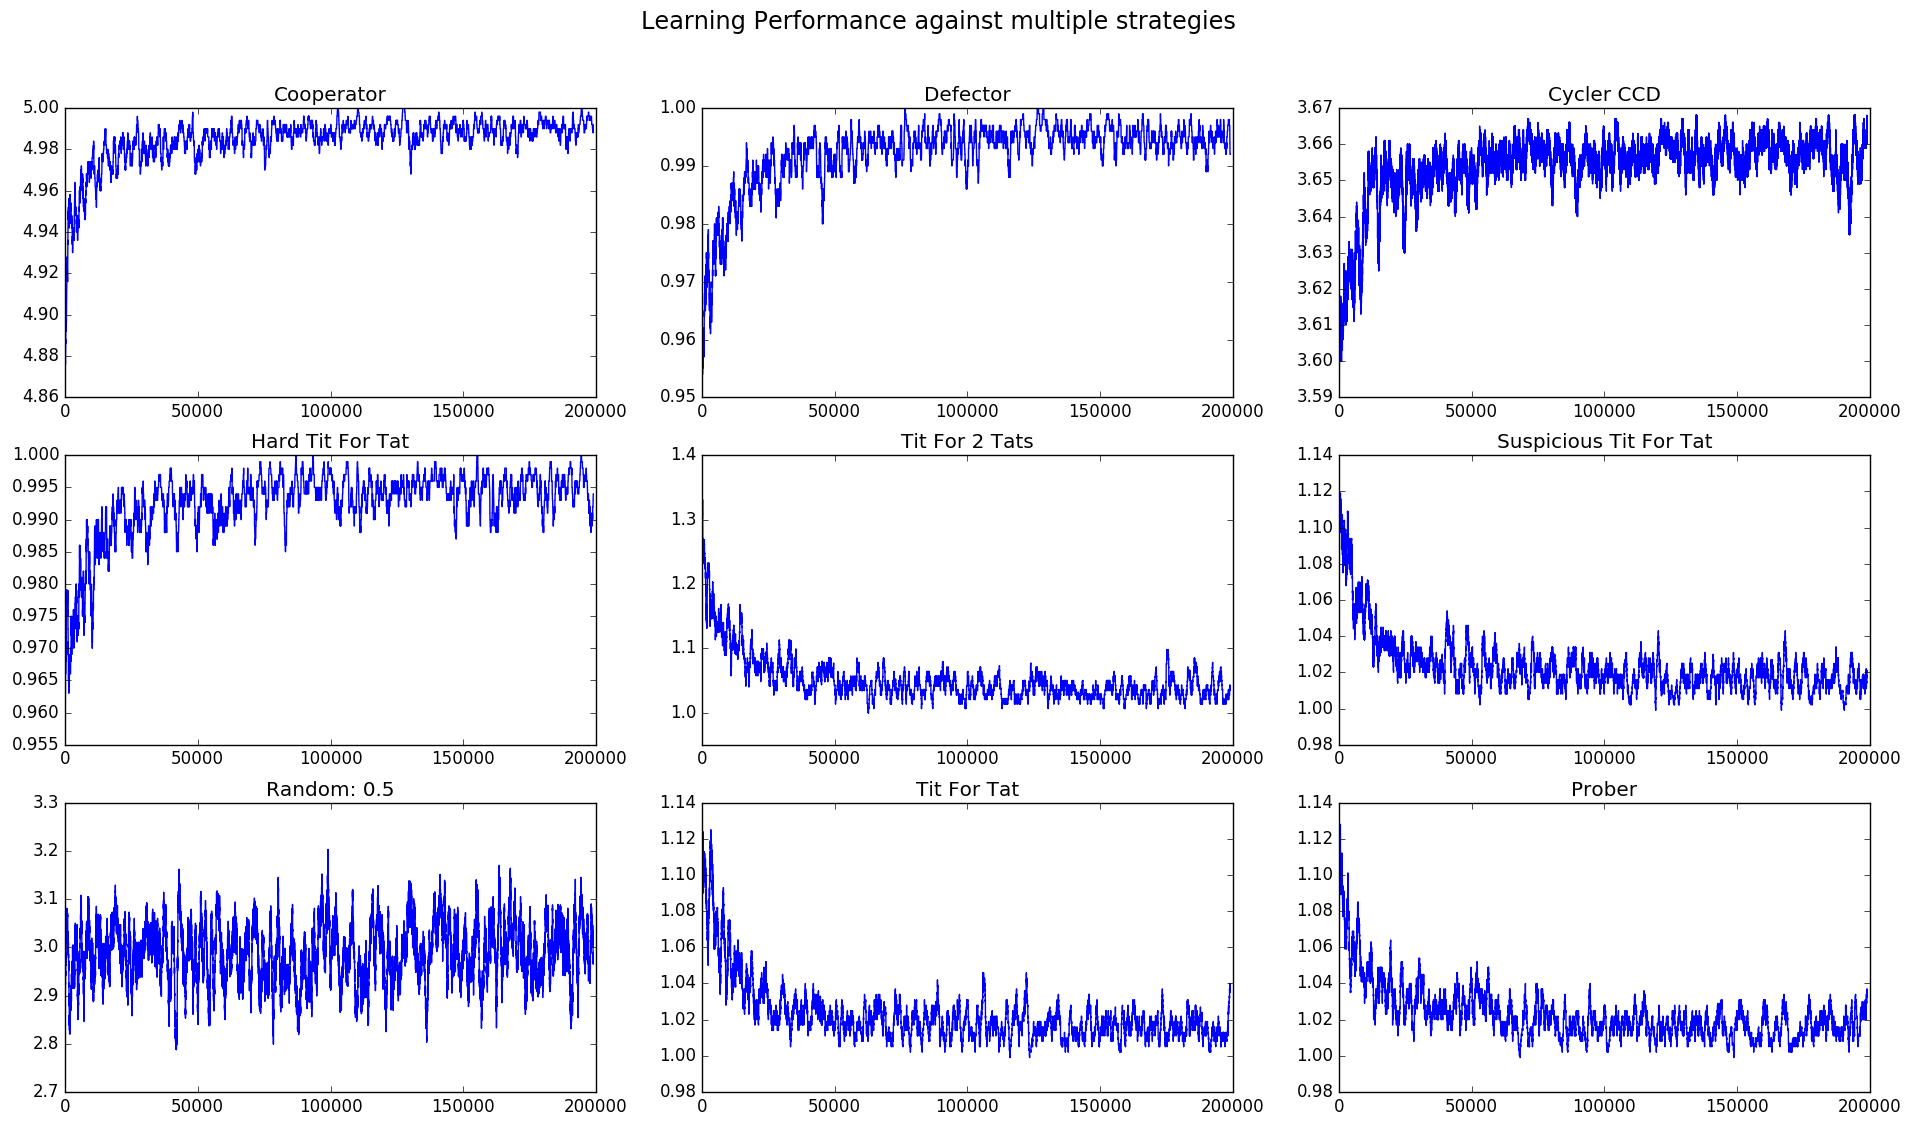
\includegraphics[width=0.9\textwidth]{learnerB.png}
	\caption{{Performance of Adaptive strategy (Variant B)}}
	\end{figure}

	\subsubsection{Initial Behavior (Payoff)}

	As discussed earlier, the proposed adaptive strategy learns the optimal way to play based on an Explore-Exploit agenda. Thus, it is critical to observe how quickly it adapts/learns to play. The following plots show the initial behavior of our adaptive strategy against multiple opponents. A gradual increase in the score is desirable. We do not show results for Variant A due to its random nature, which make the corresponding plots slightly messy.\\

	\begin{figure}[H]
	\centering
	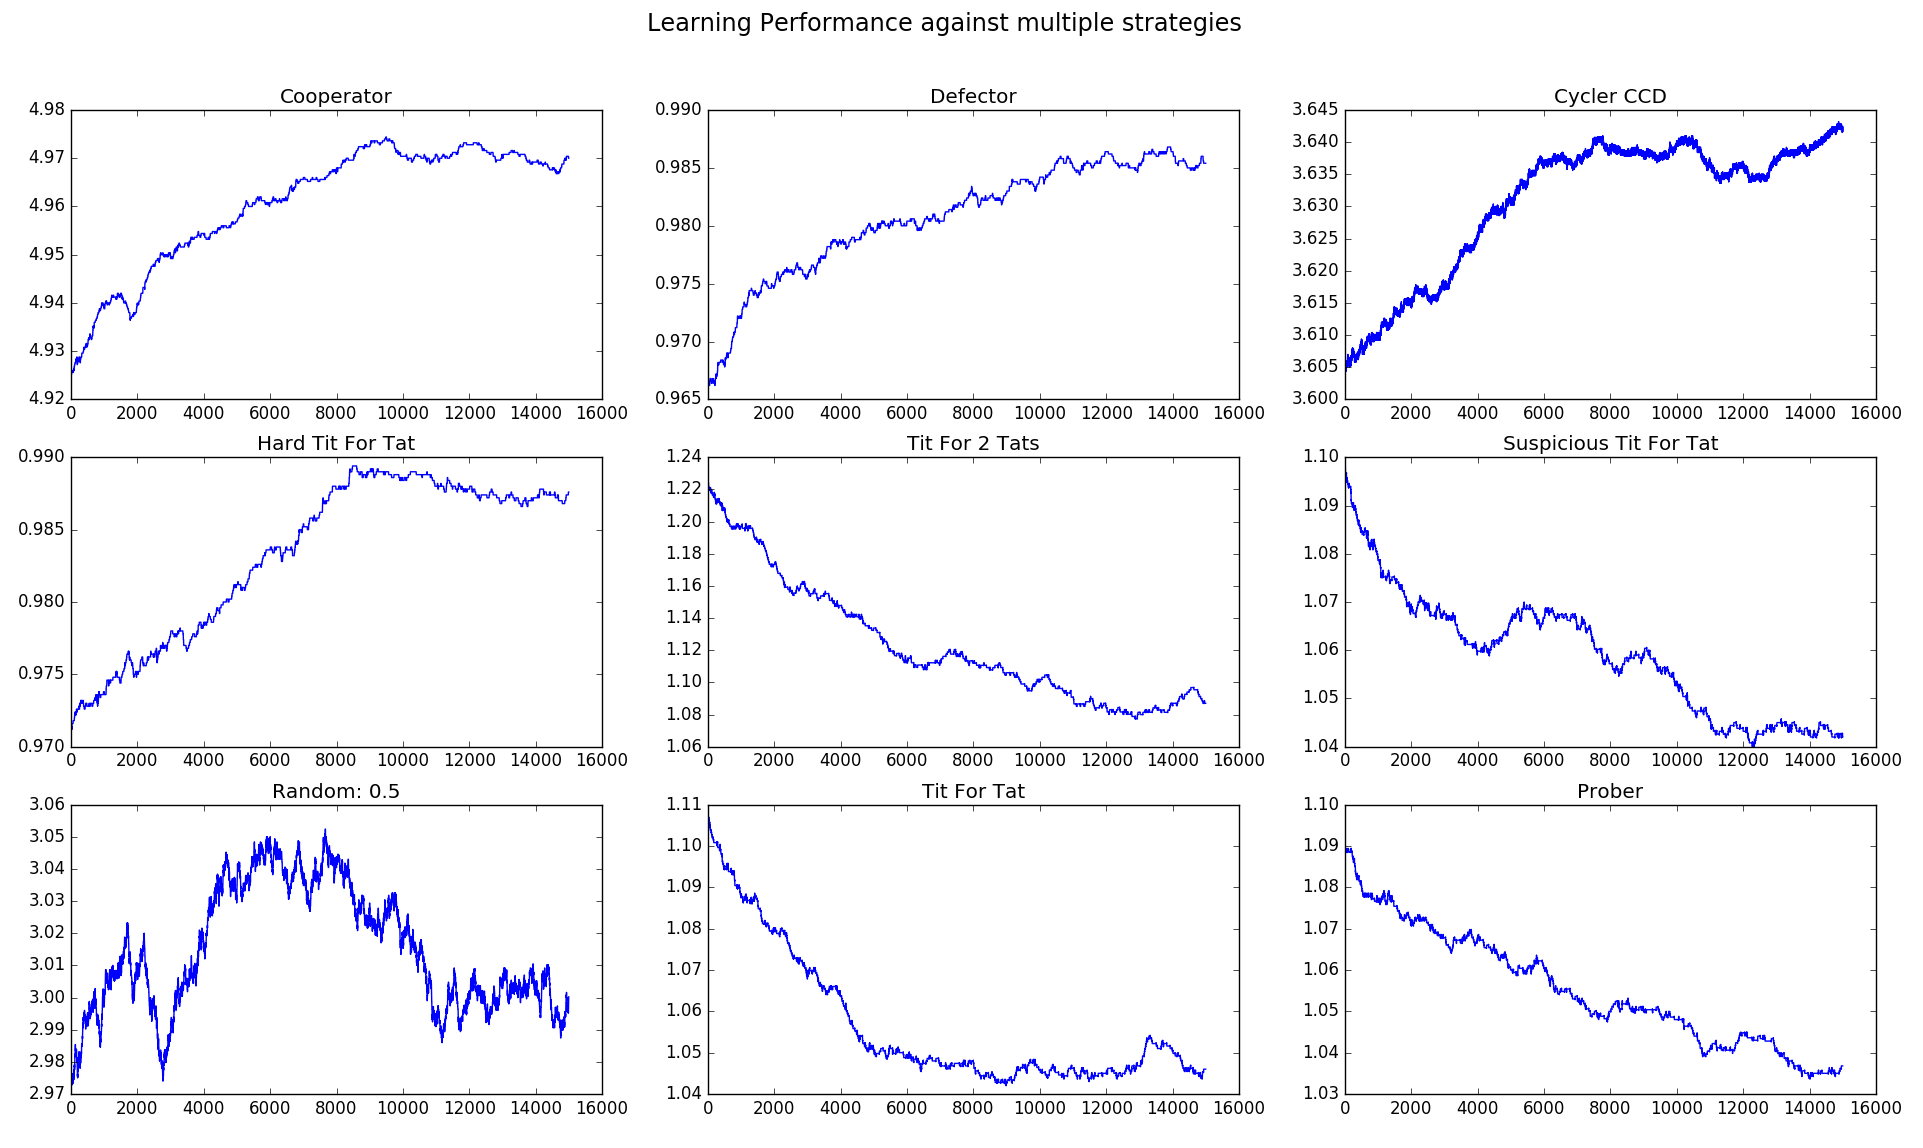
\includegraphics[width=0.9\textwidth]{learnerInitialB.png}
	\caption{{Performance of Adaptive strategy (Variant B)}}
	\end{figure}

	As we can see, our strategy generally learns and improves its payoff. But in a few cases (Mostly against 'Tit for Tat' strategies), our strategy shows a slight (Notice the scale) decreasing trend. As we will discuss later, the reason for this is poor exploration. We try to exploit more instead of exploring, which leads to a very slight decrease in the payoff (Notice the scales in the plot). The reason for this also due to only considering 'local' gains while playing (i.e. not caring about the current move on subsequent turns). This issue can be solved using a modification named as Q-Learning \cite{qlearn}.

	\begin{figure}[H]
	\centering
	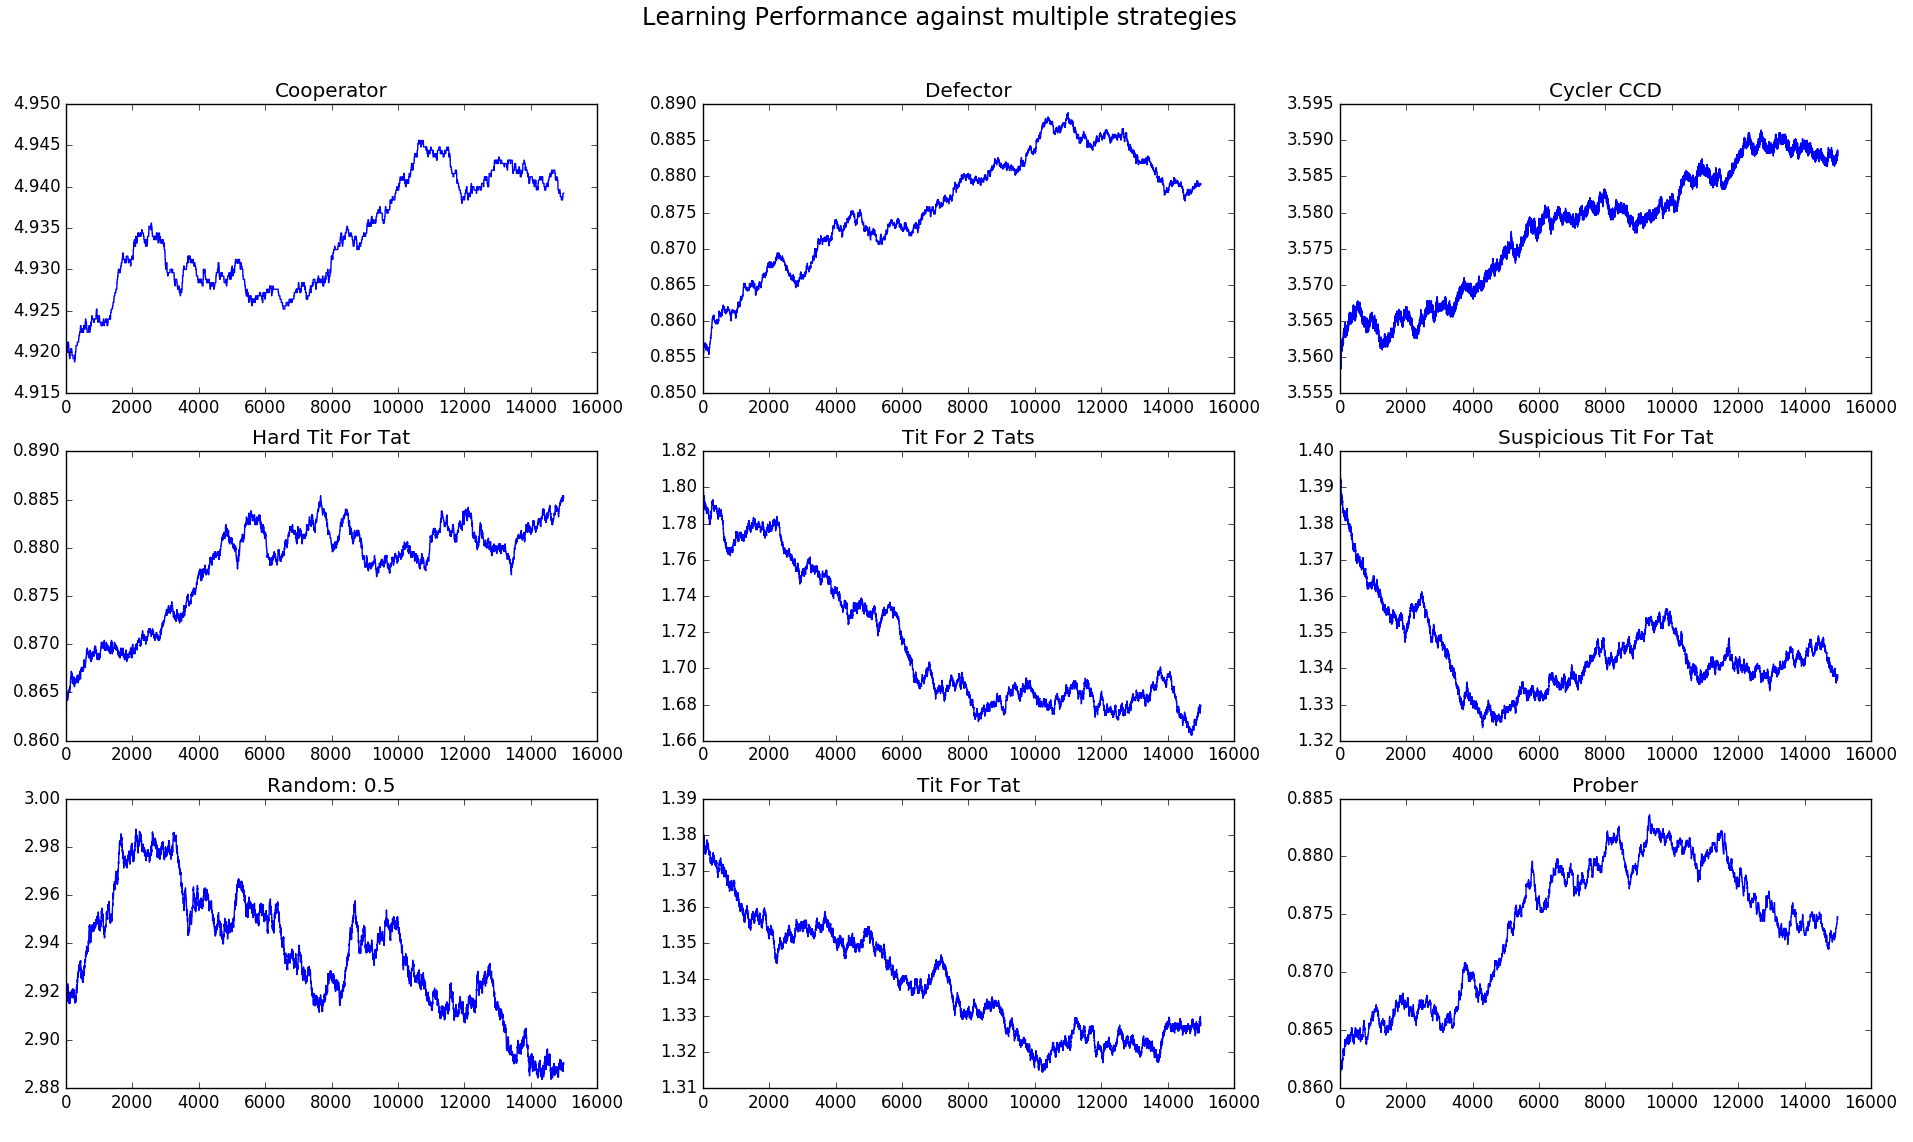
\includegraphics[width=0.9\textwidth]{learnerInitialC_b8.png}
	\caption{{Performance of Adaptive strategy (Variant C)}}
	\end{figure}

	As we can see, Variant C is able to tackle the issue of decreasing payoffs to a certain extent. We'll have a more extensive discussion on this in future sections. Using softmax to incorporate exploration at each turn helps the model in continuing to learn. The effect of the parameter $c$ which critically affects the final results id discussed later.  
	
	\subsection{Observations}
	
	We discuss the possible reasons for the behavior seen in this section. We mainly discuss the effect of $c$ (used in softmax) on the final result. This'll hopefully give us an idea about how varying the exploration strategy affects the final result. We also, try to conduct tournaments 	
	
	\subsubsection{Effect of Parameters on Learning}

	As discussed earlier, using softmax drastically helps in improving the results. Here, we study the effect of the constant $c$ on the performance of the learning algorithm. Note that, a small $c$ neglects the role of the expected payoff while a higher $c$ makes its role even more important.\\

	As we can see, for $c=2$ there is almost no decreasing trend observed (Note that the fluctuations are extremely small). This is due to more emphasis on exploration instead of exploiting the current best move. Also note the higher payoffs observed in case of 'Tit for Tat' Strategies and also the slight drop in payoffs for the others.\\
	
	With increasing $c$, the decreasing payoff effect becomes more prominent. Also, the payoffs for 'Tit for Tat' strategies decrease while it increases for the others. As mentioned earlier, this can be accounted to local greediness used by the player (i.e. not thinking about the effect of the current moves on future turns). Note that although, the payoffs are low. The adaptive strategy easily gains the highest (After defector) number of wins.

	\begin{figure}[H]
	\centering
	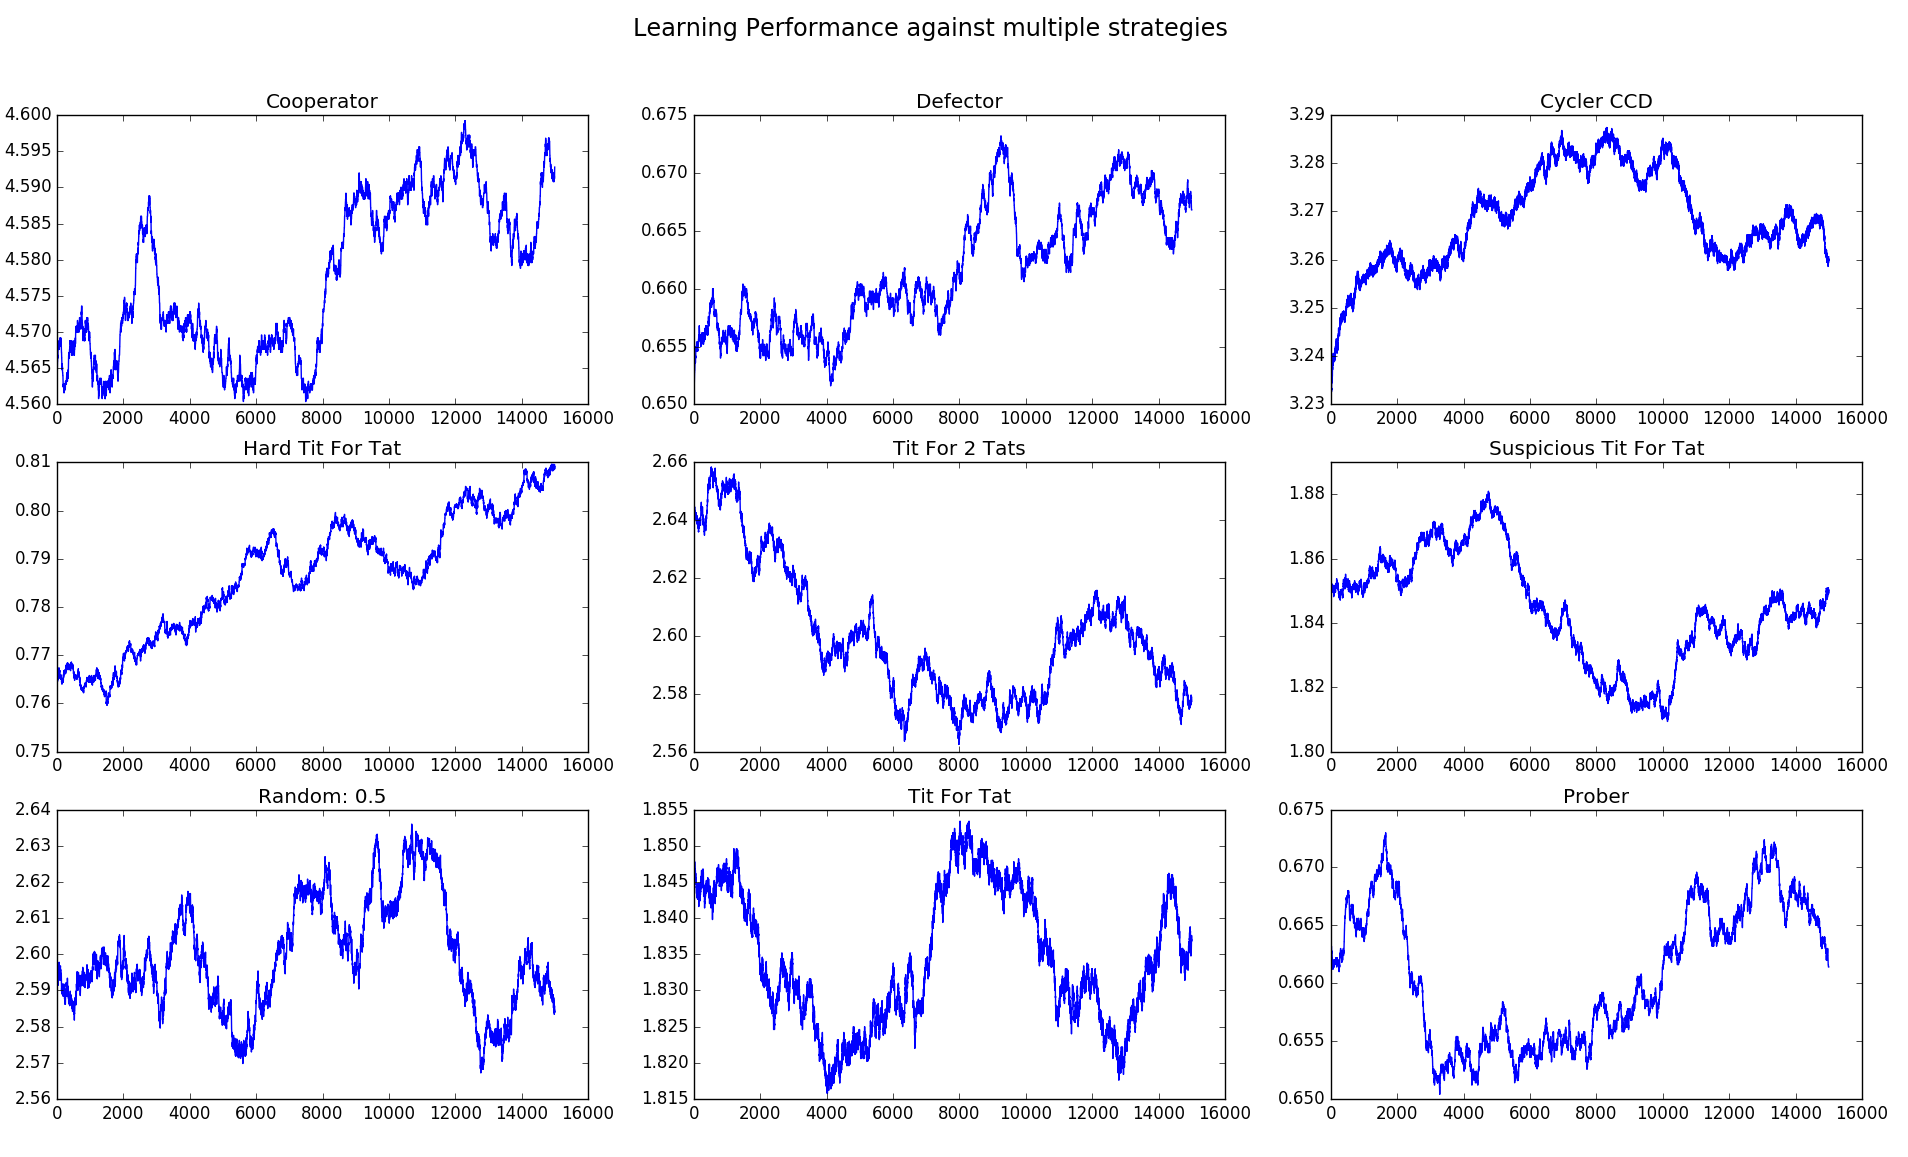
\includegraphics[width=0.73\textwidth]{learnerInitialC_b2.png}
	\caption*{{Performance of Variant C ($c = 2$)}}
	\end{figure}

	\begin{figure}[H]
	\centering
	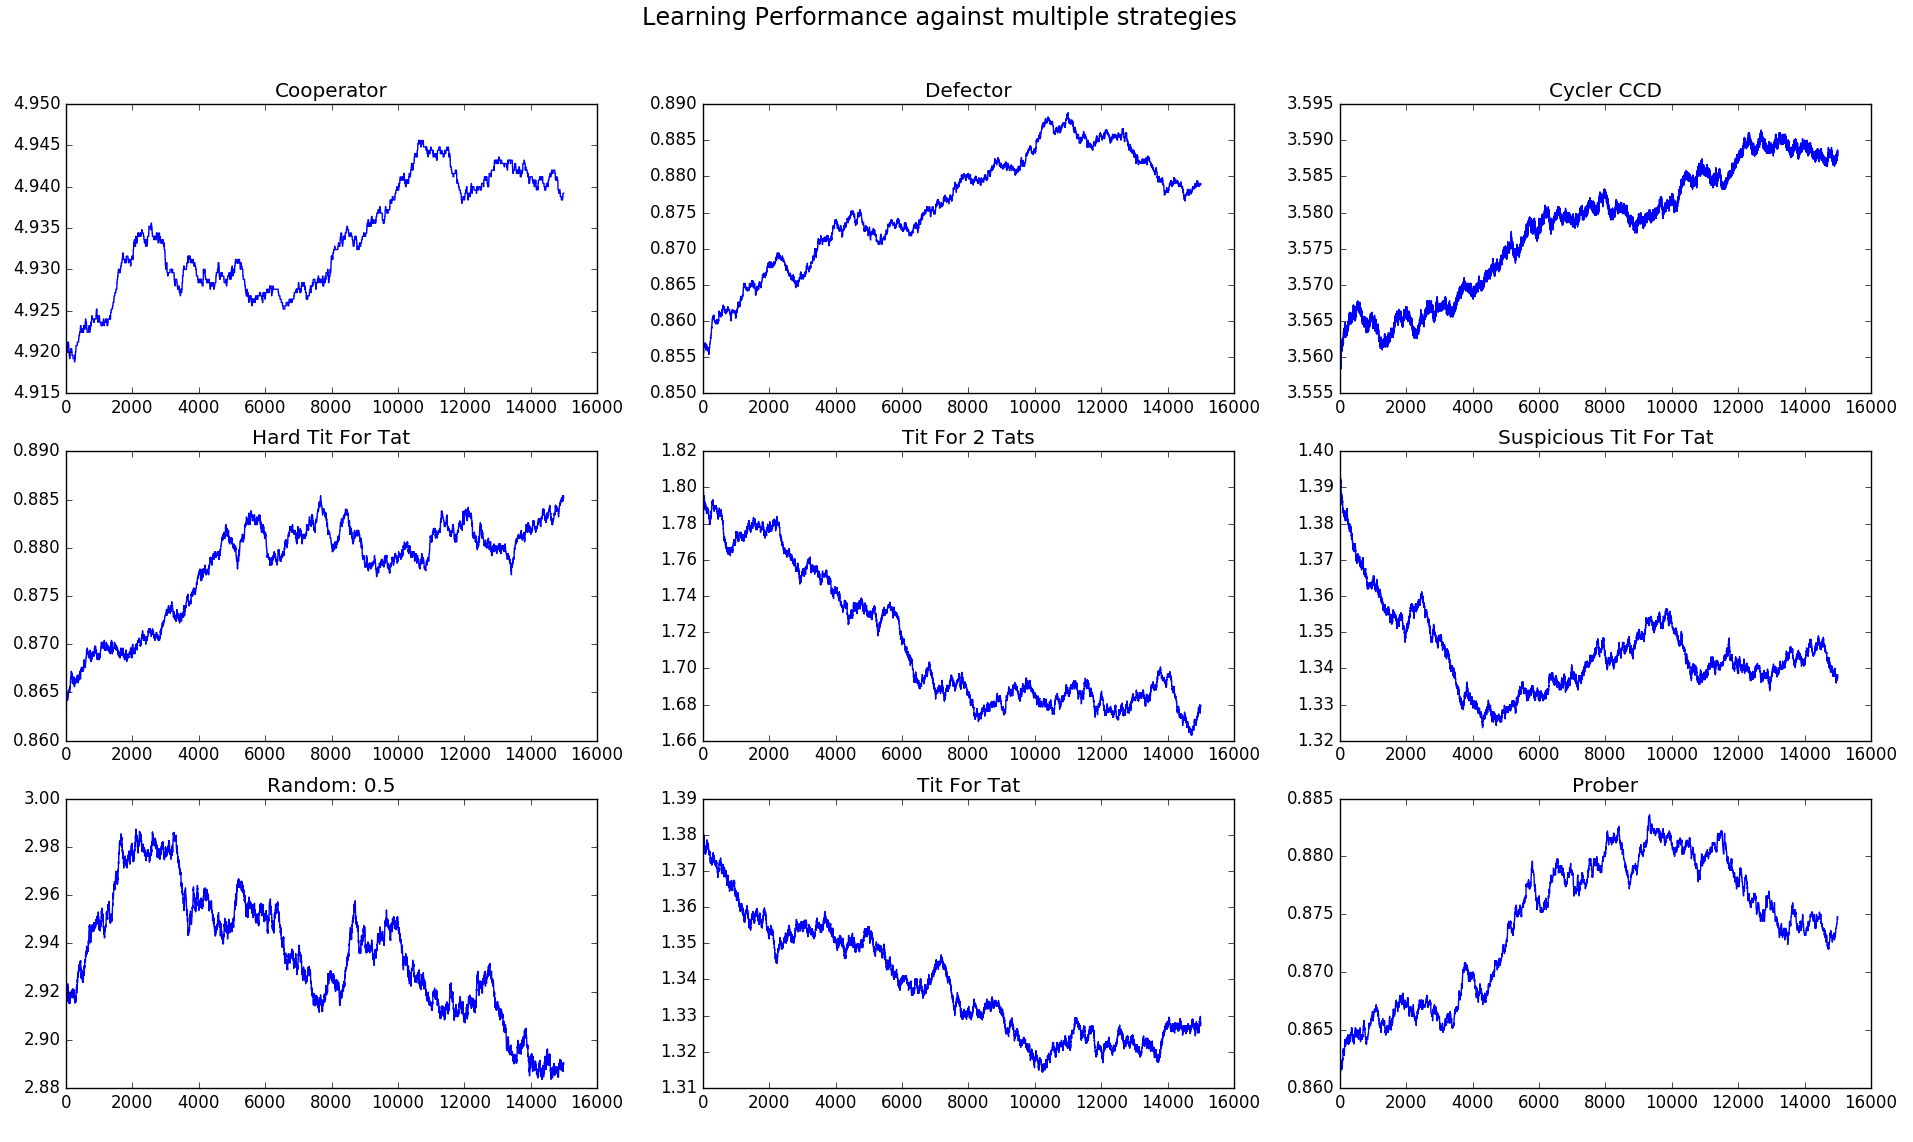
\includegraphics[width=0.73\textwidth]{learnerInitialC_b8.png}
	\caption*{{Performance of Variant C ($c = 8$)}}
	\end{figure}

	\begin{figure}[H]
	\centering
	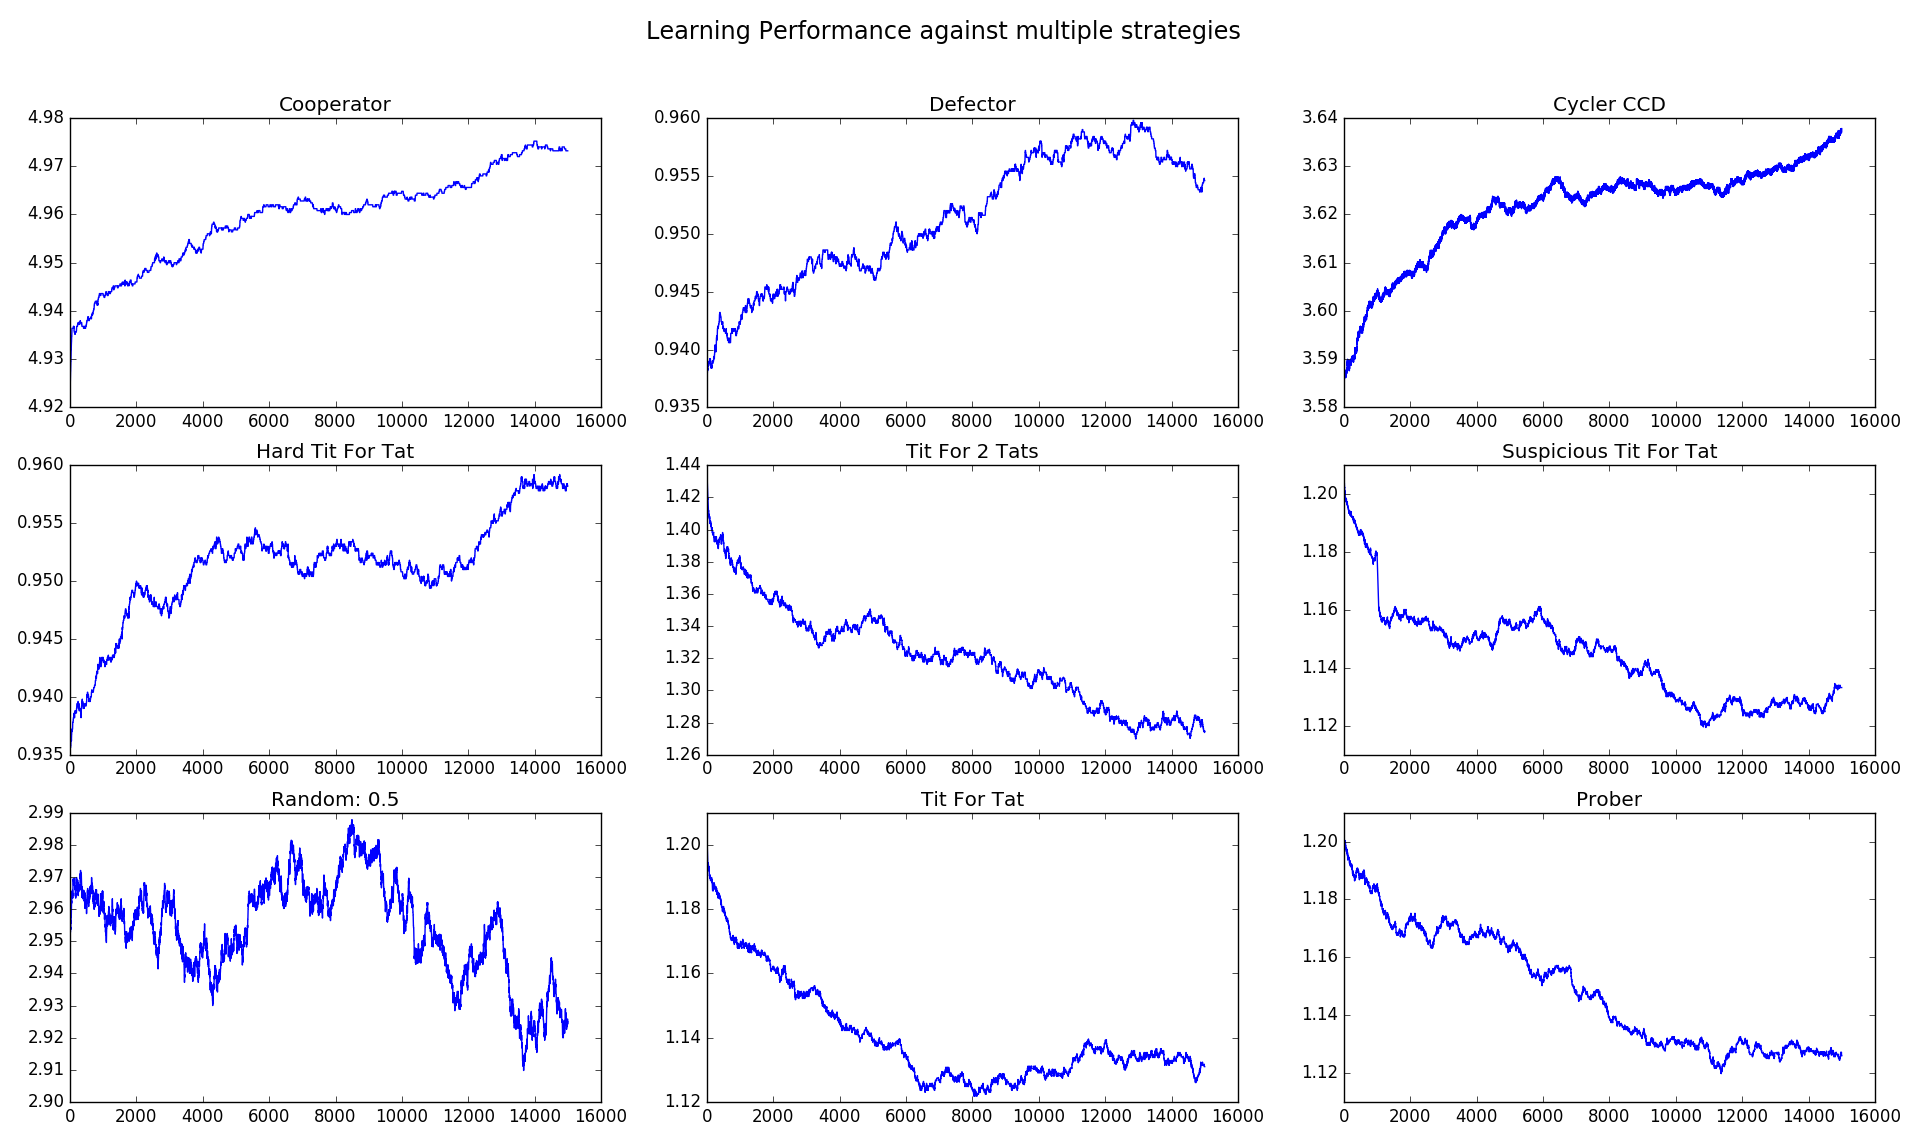
\includegraphics[width=0.73\textwidth]{learnerInitialC_b32.png}
	\caption*{{Performance of Variant C ($c = 32$)}}
	\end{figure}

	\subsubsection{Effect of Memory}
	
	Let's study the effect of memory on the performance of the adaptive strategy. It's evident that the number of states increase exponentially with memory length. Consequently, the rate of learning will also be reduced accordingly since we have a larger number of unknowns which need to be estimated. This would mean more emphasis on exploration. The performance of the strategies for different memory lengths are shown below,\\
	
	\vspace{-5mm}	
	\begin{table}[H]
	  \begin{center}
	    \begin{tabular}{|c|c|c|c|c|}
	      \toprule
		  \textsc{Memory Used} & \textsc{Cooperator} & \textsc{Defector} & {\footnotesize{\textsc{CyclerCCD}}} & \textsc{Hard TfT}\\
	      \midrule
		   1 & 	4.593 & 0.666 & 3.264 & 0.793\\
		   2 & 4.592 & 0.664 & \textbf{3.280} & 0.786\\
		   3 & 4.592 & 0.663 & \textbf{3.281} & 0.791\\
		   \bottomrule
	    \end{tabular}
	  \end{center}
	\end{table} 

	\vspace{-8mm}	
	
	\begin{table}[H]
	  \begin{center}
	    \begin{tabular}{|c|c|c|c|c|c|}
	      \toprule
	 	  \textsc{Memory Used} & \textsc{Tf2T} & {\footnotesize{\textsc{Suspicious TfT}}} & \textsc{Random} & \textsc{TfT} & \textsc{Prober}\\
	      \midrule
		  1	& 2.552 & 1.832 & 2.603 & 1.834 & 1.836\\
		  2 & \textbf{2.592} & 1.829 & 2.597 & 1.829 & 1.831\\
		  3 & \textbf{2.581} & 1.825 & 2.610 & 1.830 & 1.832\\
		\bottomrule
	    \end{tabular}
	  \end{center}
	\end{table}  		
	 
	\vspace{-5mm}	

	As we can see from the above table, increasing memory has little or almost no effect on the performance of the strategy. This can be due to the fact that almost all the above strategies are extremely local in nature (i.e. Do not look more than 1-2 steps back). Thus, only one look up is enough to explain the opposing strategies well enough. This reasoning is supported by the fact that there is a slight improvement in the payoffs of the strategies  \textsc{CyclerCCD} and \textsc{Tit for 2 Tats}, both of which require at least 2-3 memory length to tackle efficiently.\\
	
	Also note that the reinforcement learning algorithm discussed here does not look at the future implications of the current move. The related topic is Q-Learning and is extremely powerful in this sense \cite{qlearn}. Using it should help in learning future implications and subsequently gaining higher scores.
	 
	\subsubsection{Special Cases: Cooperator and Defector}

	This section discusses the performance of our proposed adaptive strategy in detail by considering selective opponents i.e. Cooperator and Defector. We select these strategies for ease of discussion.\\
	
	\noindent
	\textbf{Cooperator: } As the name suggests, this is a simple strategy which always cooperates. Our algorithm starts off in a pure state, having no knowledge of what would be a better strategy. It interacts with the opponent and slowly learns which strategy give better returns. As can be seen in earlier figures, the strategy performs poorly initially (Due to no knowledge at the moment). Initially, it tries exploring all possible moves and infer which moves should be better. Thus, as observed in the plots, the payoffs slowly start to rise and approach 5 (The optimal value). In the end, the payoff is still slightly less than 5 due to a small amount of exploration being performed (To check whether another better strategy can be found).\\
	
	\noindent
	\textbf{Defector: } As the name suggests, this is a simple strategy which always defects. Note that against such a strategy, the maximum payoff is 1. 	Similar to the previous case, our algorithm starts off by having no previous knowledge. It interacts with the opponent and slowly learns which strategy give better returns. As can be seen in earlier figures, the strategy performs poorly initially (Due to exploration being performed). Thus, as observed in the plots and noted in the previous case, the payoffs slowly start to rise and approach 1 (The optimal value). Note that a defector will always win (In any case, against any strategy other then Defector itself) and consequently will always have higher ($\geq$) payoff than the opponent. So, in effect our strategy has managed to learn the (nearly) best possible action in this case.

	\section{Showdown: Evolved Strategy Vs Adaptive Strategy}

	We perform matches between the Evolved strategies and the adaptive strategies to study their performance. We conduct matches of different length, to study both the initial and far-off behavior.
	
	\subsection{Performance Against Each Other}

	When the adaptive strategy is played against the evolved ones, the results are as follows,
	
	\begin{table}[H]
	  \begin{center}
	    \begin{tabular}{|c|c|c|}
	      \toprule
	 	  \textsc{Turns} & \textsc{Single Objective Strategy} & \textsc{Multi Objective Strategy}\\
	      \midrule
		  20    & \textbf{2.150} (1.400) & \textbf{2.400} (1.400)\\		  
		  200	& \textbf{2.190} (1.915) & \textbf{2.025} (1.725)\\
		  2000  & 1.827 \textbf{(2.017)} & 1.858 \textbf{(1.998)}\\
		  20000 & 1.781 \textbf{(1.95)} & 1.780 \textbf{(1.945)}\\
		  200000 & 1.743 \textbf{(1.962)} & 1.752 \textbf{(1.951)}\\
		\bottomrule
	    \end{tabular}
	  \end{center}
	\end{table}  		
	\vspace{-5mm}
	
	As we can see above, the adaptive strategy slowly adapts to the evolved strategy and starts outperforming them as the number of turns played increases. Note that the payoffs shown for turns = 20, 200 have extremely high variance and thus are not reliable (and should not be taken at face value).
	
	\subsection{Performance Against Other Strategies}
	
	Here, we study the performance of the discussed strategies against other players. The strategies used are a subset of those mentioned earlier.	
	
	\renewcommand{\tabcolsep}{8pt}

	\begin{table}[H]
	  \begin{center}
	    \begin{tabular}{|c|c|c|c|c|}
	      \toprule
	 	  \textsc{Strategy} & \textsc{Cooperator} & \textsc{Defector} & \textsc{CyclerCCD} & \textsc{Hard TfT}\\
		  \midrule
		  Adaptive Strategy & \textbf{4.932} \textbf{(0.102)} & 0.871 (1.514) & 3.577 (0.581) & 0.880 (1.524)\\
		  Single Obj & 4.000 (1.500) & \textbf{1.000 (1.000)} & \textbf{3.666 (0.334)} & \textbf{3.000 (3.000)}\\
		  Multi Obj & 4.000 (1.500) & \textbf{1.000 (1.000)} &  \textbf{3.666 (0.334)} & \textbf{3.000 (3.000)}\\
		\bottomrule
	    \end{tabular}
	  \end{center}
	\end{table}  		

	\vspace{-8mm}	
	\renewcommand{\tabcolsep}{6pt}

	\begin{table}[H]
	  \begin{center}
	  	\footnotesize
	    \begin{tabular}{|c|c|c|c|c|c|}
	      \toprule
	 	  \textsc{Strategy} & \textsc{Tf2T} & {\footnotesize{\textsc{Suspicious TfT}}} & \textsc{Random} & \textsc{TfT} & \textsc{Prober}\\
		  \midrule
		  Adaptive Strategy & 1.710 {(1.205)} & 1.350 (1.350) & \textbf{2.904 (0.732)} & 1.360 (1.360) & 1.340 (1.340)\\
		  Single Obj & \textbf{4.000} \textbf{(1.500)} & \textbf{3.000 (3.000)} & 2.487 (1.710) & \textbf{3.000 (3.000)} & \textbf{3.000 (3.000)}\\
		  Mult Obj & \textbf{4.000} \textbf{(1.500)} & \textbf{3.000 (3.000)} & 2.488 (1.712) & \textbf{3.000 (3.000)} & \textbf{3.000 (3.000)}\\
		  \bottomrule
	    \end{tabular}
	  \end{center}
	\end{table}  		
	\vspace{-3mm}	

	As we can see here, the adaptive strategy performs well or comparable in case of strategies such as Cooperator, Defector, CyclerCCD and Random. But it almost constantly performs poor in case of 'Tit for Tat' type strategies. A highly possible reason for this could be the fact that the solution search is extremely local (And thus we do not focus on the future of the game). Q-Learning \cite{qlearn} is a possible solution for the same.

	It should be mentioned that the above experiment is extremely unfair towards the Adaptive strategy. Since the evolved strategies have been trained on the given strategies. In case of completely new strategies, the evolved ones perform very poorly compared to the adaptive algorithm (Results have not been shown due to space constraints).

	\section{Significance of the Results}
	
	We see that evolved strategies perform well in general but that only holds true against known strategies. We can conclude the following features of the Evolved Strategies on the basis of the above discussions,
	\begin{itemize}
		\item \textbf{High Performance:} Evolved strategies perform extremely well (In terms of average payoff) against known strategies (i.e. strategies against which they've been trained).
		\item \textbf{Poor Performance against Fresh Opponents:} Evolved strategies perform vwey poorly against fresh strategies. Mainly due to there rigid strategies which aren't able to adapt to the new strategies.
		\item \textbf{Low Win Rate:} In the round robin tournament conducted, it was observed that even though the scores obtained by the evolved strategies were high. They were not able to win a large number of games. Their final position was around $5^{th}-6^{th}$ out of 11 players.
		\item \textbf{Fixed Behavior:} It is evident that the evolved strategies are rigid in nature and do not change their behavior on the basis of the opponent. Which is a desirable quality in a strategy.
	\end{itemize}

	We can observe the following features of the Adaptive Strategies,
	\begin{itemize}
		\item \textbf{Varying Performance:} Adaptive strategies sometimes perform extremely well (In some cases, being able to exploit the optimal strategy) against some strategies. While in case of others, their average return isn't that high and they lose to evolved strategies. But an important point to note is that even thought their returns are low, they manage to win most of the games. More discussion in the latter points.
		\item \textbf{Poor Performance against 'Tit for Tat' strategies:} It can be seen in the results that the payoffs are low for 'Tit for Tat' class of strategies. But, it still manages to win finally. The low payoff can be rectified by using Q-Learning (A variant which considers the effect on future moves).
		\item \textbf{Robust against Fresh Opponents:} Unlike the Evolved strategies, adaptive strategies manage to learn the best (good) way to play against new opponents.
		\item \textbf{High Win Rate:} In the round robin tournament conducted, it was observed that even though the scores obtained by the Adaptive Strategy was moderate. It was able to win a majority of games. Its final position was $2^{nd}$ out of 11 players. Only coming behind 'Defector' which as discussed earlier can not be defeated.	
		\item \textbf{Adaptive Behavior:} As the name suggests, this strategy adapts well to new opponents. Which is an extremely desirable quality in a strategy.
		\item \textbf{Gradual Increase in Performance:} It is natural that the strategy performs poorly initially but then its performance improves as the number of turns progresses.				
	\end{itemize}		
	
	\section{Conclusion}	
			
	We have confirmed known results and findings related to Infinite Prisoner's Dilemma (By Axelrod). We also propose a few changes in the list of desirable traits given by Axelrod, alongside confirming their relevance in high performing strategies. We also show the relevance of choosing memory depth as three in experiments and provide a loose argument to support it. After discussing the flaws associated with evolved strategies, we also propose new adaptive algorithms based on reinforcement learning to counter them. We study the performance of the discussed strategies by conducting various experiments. We use a similar setup (As done by Axelrod) to decide the effectiveness of the computed strategies. We also mention the superiority of the adaptive strategies against fresh strategies which is a weak point for evolved strategies. Hopefully, the improvements an correction suggested (Such as Q-Learning) helps the adaptive strategy obtain high payoffs against those which it is currently weak against.
					
	\pagebreak					
					
	\section{References}

	\bibliographystyle{plain}

	\bibliography{sources}	

\end{document}


